% The earlier collision record at the 31 locations where a cyclist was killed, Montréal 2012–2021 (SPVM open data).
% Built by build.py (tables regenerated from the CSVs, version stamped, pdflatex twice).
\documentclass[11pt,letterpaper]{article}
\usepackage[T1]{fontenc}
\usepackage[utf8]{inputenc}
\usepackage[scaled=0.95]{helvet}
\renewcommand{\familydefault}{\sfdefault}
\usepackage[letterpaper,top=0.9in,bottom=0.95in,left=0.9in,right=0.9in]{geometry}
\usepackage{microtype}
\usepackage{enumitem}
\usepackage{titlesec}
\usepackage{fancyhdr}
\usepackage{xcolor}
\usepackage{booktabs}
\usepackage{longtable}
\usepackage{seqsplit}
\usepackage{amsmath}
\usepackage{graphicx}
\usepackage{array}
\usepackage[hidelinks]{hyperref}
\usepackage{url}\def\UrlBreaks{\do\_\do\-}
\newcommand{\code}[1]{\texttt{\seqsplit{#1}}}
\urlstyle{same}
\newcommand{\docversion}{2026-10-26-22-33-15} % set by build (America/Toronto)
\hypersetup{pdfsubject={version \docversion}}

\setlength{\parindent}{0pt}
\setlength{\parskip}{0.5em}
\linespread{1.03}

\titleformat{\section}{\normalfont\large\bfseries}{\thesection}{0.6em}{}[\vspace{1pt}\titlerule]
\titlespacing*{\section}{0pt}{1.1em}{0.4em}
\titleformat{\subsection}{\normalfont\bfseries}{\thesubsection}{0.6em}{}
\titlespacing*{\subsection}{0pt}{0.8em}{0.25em}

\pagestyle{fancy}
\fancyhf{}
\renewcommand{\headrulewidth}{0pt}
\fancyfoot[C]{\footnotesize\color{gray}Montreal-collisions -- the earlier record and later deaths, 2012--2021 -- page \thepage}
\fancyfoot[R]{\tiny\color{gray}v.\,\docversion}

\newcommand{\repourl}{https://github.com/OpenMobilityData/Montreal-collisions}
\newcommand{\repo}[1]{\href{\repourl}{#1}}
\newcommand{\doc}[2]{\href{\repourl/blob/main/#1}{#2}}

\begin{document}

{\LARGE\bfseries Does the earlier record at a location predict a later death?}

{\large Montréal 2012--2021, police-reported collisions (SPVM open data): the record of 2012--2016 at every 100\,m cell against the cyclist and pedestrian deaths of 2017--2021}

\medskip
Data note, October 26, 2026. Repository: \repo{\repourl}. Version \docversion. Companion to \doc{derived/cyclist-fatality-locations/}{\emph{Before a cyclist was killed}}.

\section*{Summary}

The companion note found that at 30 of the 31 locations where a cyclist was killed in 2012--2021, no fatal collision of any kind had been recorded nearby before. This note asks the other half of the question: whether the \emph{volume} of the earlier record at a place, fatal or not, goes with a later death. The territory is cut into 100\,m cells on the City's coordinates; for the 17,593 cells with at least one police-reported collision in 2012--2016, the record of those five years (all collisions, injury collisions, collisions with a bicycle, with a pedestrian victim) is set against the deaths of 2017--2021: 13 collisions in which a cyclist was killed, 87 in which a pedestrian was killed.

\textbf{The earlier record does go with later deaths, in the aggregate. Most cells record no injury collision in five years, and the death sites sit around the 90th percentile of the earlier record (Table~\ref{tab:pct}). Ranked by their 2012--2016 injury collisions, the top tenth of cells (1,759 cells) held 6 of the 13 cyclist deaths and 53 of the 87 pedestrian deaths of 2017--2021; the bottom seven tenths (12,316 cells) held 1 and 13 (Table~\ref{tab:dec}). What the record cannot do is name the place: a cell in the top tenth saw a cyclist killed in one case in about 300 over five years, a pedestrian in one in 33; flagging that tenth catches 46\,\% of the cyclist deaths and 61\,\% of the pedestrian deaths, and catching five in six takes the top 30\,\%, some 5,300 cells (Table~\ref{tab:top}).} The picture is the same with 200\,m cells and with the split moved a year earlier (Table~\ref{tab:sens}).

Rue de Terrebonne on the same scale (Table~\ref{tab:terr}): the cell at avenue Girouard recorded 20 collisions and 11 with an injury in 2012--2016, the 97.6th percentile of all cells, in the top tenth; the pedestrian death of September 3, 2019 fell in that cell. The street's other intersections sit between the 46th and the 89th percentile; of the 20 cells along the lane's axis with a record before 2017, one (Girouard) is in the top tenth.

No measure of exposure enters these tables: the earlier record of a cell rises with the traffic, the cycling and the walking that pass through it, and the association measured here is between a busy record and a later death, not between any feature of the place and the death.

\section{Data and units}

The SPVM open-data file of police-reported collisions 2012--2021 (218,272 rows; 218,261 with coordinates), as described in the companion note and the repository README. Each located collision is assigned to the 100\,m square of the City's MTM zone~8 grid containing its point (200\,m squares as a check). A square is a crude unit: it cuts some intersections in two and joins others; it is the same for every place and needs no choice of intersections. The \emph{before} window is 2012--2016 and the \emph{after} window 2017--2021; the check moves the split to 2016. A death is a collision with \code{NB\_DECES\_VELO} $>$ 0 (cyclist) or \code{NB\_DECES\_PIETON} $>$ 0 (pedestrian); an injury collision has \code{GRAVITE} \emph{Mortel}, \emph{Grave} or \emph{Léger}.

\section{Method}

For every cell with at least one collision in the before window: the before record (all, injury, bicycle, pedestrian, fatal) and the after outcome (cyclist deaths, pedestrian deaths). Three readings:
\begin{enumerate}[leftmargin=1.6em]
\item \textbf{Were the death sites ordinary?} For each death of the after window at a cell with a before record, the percentile of that cell's before record among all cells with a record (one entry per death; four measures of the record). Deaths at cells with no before record (1 cyclist, 2 pedestrians) are counted and set aside.
\item \textbf{Does the before record predict a death?} Cells ranked by before injury collisions (ties by all collisions, then at random with a fixed seed) and cut into ten equal deciles; deaths per 100 cells by decile with exact Poisson 95\,\% intervals.
\item \textbf{What would flagging the busiest cells have caught?} The share of after-window deaths in the top 1, 2, 5, 10, 20, 30 and 50\,\% of cells by the same ranking.
\end{enumerate}
Everything is produced by \doc{scripts/location\_record\_test.py}{scripts/location\_record\_test.py} from the loader \doc{scripts/spvm.py}{scripts/spvm.py}; the tables are the CSV files beside this note, and \code{decile\_chart.py} draws Figure~\ref{fig:dec}.

\section{Results}

\begin{figure}[htbp]\centering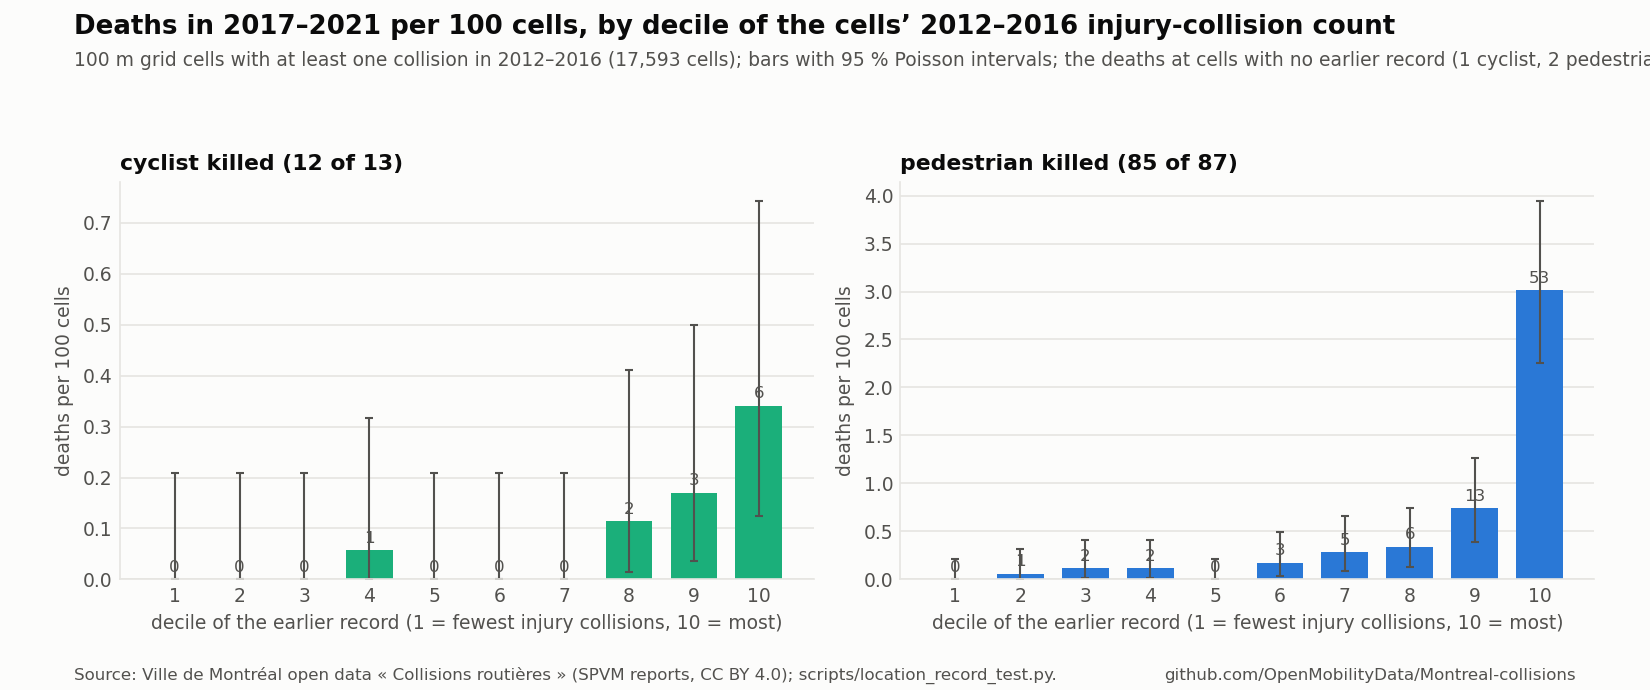
\includegraphics[width=\linewidth]{deaths_by_decile_en.png}
\caption{Deaths of 2017--2021 per 100 cells by decile of the cells' 2012--2016 injury-collision count, with 95\,\% Poisson intervals; the number on each bar is the count of deaths.}\label{fig:dec}\end{figure}

% generated by build.py
\begin{table}[htbp]\centering\caption{Where the death sites of 2017--2021 sit in the distribution of the 2012--2016 record of all 100\,m cells with a record (17,593 cells): median percentile of the death sites, and the share of deaths at sites in the top tenth, the top quarter and the lower half. One cyclist death and two pedestrian deaths fell in cells with no earlier record and are outside the ranking.}\label{tab:pct}
\footnotesize\begin{tabular}{@{}l l r r r r@{}}\toprule Deaths & Earlier record measured as & Median percentile & Top tenth & Top quarter & Lower half\\ \midrule
cyclist killed (12 of 13) & all collisions & 91.8 & 58\,\% & 67\,\% & 8\,\%\\
cyclist killed (12 of 13) & injury collisions & 89.9 & 50\,\% & 92\,\% & 0\,\%\\
cyclist killed (12 of 13) & collisions with a bicycle & 95.0 & 75\,\% & 100\,\% & 0\,\%\\
cyclist killed (12 of 13) & collisions with a pedestrian victim & 82.1 & 42\,\% & 100\,\% & 0\,\%\\
pedestrian killed (85 of 87) & all collisions & 90.8 & 60\,\% & 84\,\% & 7\,\%\\
pedestrian killed (85 of 87) & injury collisions & 93.0 & 65\,\% & 91\,\% & 0\,\%\\
pedestrian killed (85 of 87) & collisions with a bicycle & 95.0 & 64\,\% & 100\,\% & 0\,\%\\
pedestrian killed (85 of 87) & collisions with a pedestrian victim & 93.5 & 68\,\% & 100\,\% & 0\,\%\\
\bottomrule\end{tabular}\end{table}

\begin{table}[htbp]\centering\caption{Deaths in 2017--2021 per 100 cells by decile of the cells’ 2012--2016 injury-collision count (ties broken by the count of all collisions, then at random with a fixed seed), with 95\,\% Poisson intervals. 100\,m cells, 1,759 or 1,760 per decile.}\label{tab:dec}
\footnotesize\begin{tabular}{@{}r r r r r r r@{}}\toprule Decile & Injury collisions 2012--2016 & \multicolumn{2}{c}{Cyclist killed} & \multicolumn{2}{c}{Pedestrian killed}\\ & (min--max) & deaths & per 100 cells (95\,\% CI) & deaths & per 100 cells (95\,\% CI)\\ \midrule
1 & 0--0 & 0 & 0.00 (0.00--0.21) & 0 & 0.00 (0.00--0.21)\\
2 & 0--0 & 0 & 0.00 (0.00--0.21) & 1 & 0.06 (0.00--0.32)\\
3 & 0--0 & 0 & 0.00 (0.00--0.21) & 2 & 0.11 (0.01--0.41)\\
4 & 0--0 & 1 & 0.06 (0.00--0.32) & 2 & 0.11 (0.01--0.41)\\
5 & 0--0 & 0 & 0.00 (0.00--0.21) & 0 & 0.00 (0.00--0.21)\\
6 & 0--1 & 0 & 0.00 (0.00--0.21) & 3 & 0.17 (0.04--0.50)\\
7 & 1--1 & 0 & 0.00 (0.00--0.21) & 5 & 0.28 (0.09--0.66)\\
8 & 1--2 & 2 & 0.11 (0.01--0.41) & 6 & 0.34 (0.13--0.74)\\
9 & 2--4 & 3 & 0.17 (0.04--0.50) & 13 & 0.74 (0.39--1.26)\\
10 & 4--81 & 6 & 0.34 (0.13--0.74) & 53 & 3.01 (2.26--3.94)\\
\bottomrule\end{tabular}\end{table}

\begin{table}[htbp]\centering\caption{Share of the 2017--2021 deaths that fell in the cells ranked in the top $k$\,\% by their 2012--2016 record (deaths at cells with no earlier record count as not caught).}\label{tab:top}
\footnotesize\begin{tabular}{@{}r r r r@{}}\toprule Top $k$\,\% of cells & Cells flagged & Cyclist deaths caught (of 13) & Pedestrian deaths caught (of 87)\\ \midrule
1 & 175 & 3 (23\,\%) & 9 (10\,\%)\\
2 & 351 & 4 (31\,\%) & 17 (20\,\%)\\
5 & 879 & 5 (38\,\%) & 31 (36\,\%)\\
10 & 1,759 & 6 (46\,\%) & 53 (61\,\%)\\
20 & 3,518 & 9 (69\,\%) & 66 (76\,\%)\\
30 & 5,277 & 11 (85\,\%) & 72 (83\,\%)\\
50 & 8,796 & 11 (85\,\%) & 80 (92\,\%)\\
\bottomrule\end{tabular}\end{table}

\begin{table}[htbp]\centering\caption{The same quantities with 200\,m cells and with the split moved one year earlier: deaths in the top decile and in the bottom seven deciles, and the median percentile of the death sites (earlier record = injury collisions).}\label{tab:sens}
\footnotesize\setlength{\tabcolsep}{4pt}\begin{tabular}{@{}l r r r r r r@{}}\toprule Windows & Cell & \multicolumn{2}{c}{Cyclist killed} & \multicolumn{2}{c}{Pedestrian killed} & Median percentile\\ & & top decile & bottom seven & top decile & bottom seven & cyclist / pedestrian\\ \midrule
2012-2016 | 2017-2021 & 100\,m & 6 of 13 & 1 & 53 of 87 & 13 & 89.9 / 93.0\\
2012-2016 | 2017-2021 & 200\,m & 6 of 13 & 2 & 43 of 87 & 16 & 90.1 / 91.3\\
2012-2015 | 2016-2021 & 100\,m & 6 of 15 & 2 & 57 of 103 & 16 & 88.4 / 93.5\\
2012-2015 | 2016-2021 & 200\,m & 8 of 15 & 3 & 50 of 103 & 17 & 91.0 / 89.4\\
\bottomrule\end{tabular}\end{table}

\begin{table}[htbp]\centering\caption{Rue de Terrebonne on the same scale: the 2012--2016 record of the 100\,m cell holding each intersection, and its percentile among the 17,593 cells with a record.}\label{tab:terr}
\footnotesize\begin{tabular}{@{}l r r r r r r r@{}}\toprule Intersection & All & Injury & Bicycle & Pedestrian & Percentile (all) & Percentile (injury) & Top tenth\\ \midrule
Terrebonne / Girouard & 20 & 11 & 3 & 2 & 92.5 & 97.6 & yes\\
Terrebonne / Draper & 0 & 0 & 0 & 0 & -- & -- & no\\
Terrebonne / Royal & 5 & 1 & 1 & 0 & 69.8 & 76.7 & no\\
Terrebonne / Grand & 2 & 0 & 0 & 0 & 46.3 & 56.7 & no\\
Terrebonne / Kensington & 5 & 0 & 0 & 0 & 69.8 & 56.7 & no\\
Terrebonne / Cavendish & 14 & 1 & 0 & 1 & 88.6 & 76.7 & no\\
Terrebonne / King Edward & 4 & 2 & 0 & 0 & 64.3 & 84.3 & no\\
\bottomrule\end{tabular}\end{table}


\section{Limits}

\begin{itemize}[leftmargin=1.2em]
\item \textbf{No exposure.} Cycling and walking volumes are not in the file. A busy record is largely a busy place; the tables do not separate the two, and say nothing about the design of any place.
\item \textbf{Few deaths.} Thirteen cyclist deaths in the after window give a direction, with wide intervals (Table~\ref{tab:dec}); the pedestrian series carries the statistical weight. The two series agree.
\item \textbf{Units and windows are choices.} Squares cut intersections; the split date is arbitrary. The 200\,m and the earlier-split checks give the same picture (Table~\ref{tab:sens}).
\item \textbf{Record, not risk.} The file holds collisions reported to the police on the SPVM's territory; the two property-damage classes changed in volume after 2013, which is why the ranking uses injury collisions.
\item \textbf{A record of who was riding.} Cycling in Montréal, and winter cycling in particular, grew over the window and after it (the City's winter counts rose from about 2018, and the REV network opened from 2020). A quiet record on a street in the early years says as much about how few people rode there as about the street, and nothing about the years after 2021, which the file does not cover.
\item \textbf{One record, one city, one decade.} The result is a description of this file, not a general law.
\end{itemize}

\section*{About}

Written by Rick Hoge, a resident of Côte-des-Neiges--Notre-Dame-de-Grâce, from the City's open data, as a private citizen. Corrections through the repository's issue tracker.

\end{document}
